\documentclass[11pt,a4paper]{article}
\usepackage[utf8]{inputenc} 
\usepackage{graphicx} 
\usepackage[left=2cm,top=2cm,right=2cm,bottom=1.5cm]{geometry}
\usepackage{amsmath} %for mathThe WS\_2017 Game \\
\usepackage{fancyhdr}
\usepackage{listings} %for code
\usepackage{hyperref}
\usepackage{float}

\pagestyle{fancy}


\lhead{The WS\_2017 Game \\ Programm Architecture}
\rhead{Flavia Brogle \\
	 Max Hackinger}
\cfoot{\thepage}

\title{The WS\_2017 Game \\ The Programm Architecture}
\author{Flavia Brogle \\ Max Hackinger}

\renewcommand{\headrulewidth}{0.4pt}
\renewcommand{\footrulewidth}{0.4pt}
\begin{document}

	\maketitle
  \tableofcontents
  
\begin{abstract}
  This article describes the Program Architecture of the WS\_2017 Game, starting with a quick overview of all the  software components of Game. In the next three sections it goes in to grater detail about how the Client and Server side are constructed and how they communicate.
\end{abstract}  
  \clearpage
	\section{Quick over view of the Game Program}
	  WS\_2017 is a round based game that consists of a clients and a server which communicate through the WS\_2017 protocol. The protocol is inspired by the design of the POP3 protocol and uses commands that consist of a keyword and arguments.

	\section{Client side}
		\subsection{Chats and Main Window}
We created our own ChatPanel Class which can be used as different kinds of Chats in different Windows. When created the chat command is defined (chatm, chatl or chatw) so it can be used for the three different chat-types there are in our game:
- the Main Chat with all the logged-in users,
- the Lobby Chat of which one exists per game and
- the Whisper Chat with which users can privately chat.
The Main Window is one of the biggest Classes which holds the List of all the Games on the Client Side (directly in the JList in which they are displayed) and the users. This way we avoid possible bugs where a game is shown which doesn't exist anymore.
All the interaction is read in from the window. It is not directly processed but sent to the server and every client relevant to the information (i.e. the two clients in a whisper chat) including the one which received the user input get the update from the server and only then it is processed.

		\subsection{Lobby}
		When a client joins a game the lobby window is automatically opened in which all the players in this game can chat with each other. Additionally another window is created where the client can choose the Children. The Children are handled as JPanels which hold JComponents to customize the Child. When pressing the okay button the window class transforms the information about the children in a string and gives it to the GameController via server.
		\subsection{}
	\section{Server side}
		\subsection{Game State and Connection Handling}
		When a server instance is first spun up, a main thread is crated that in turn spins up a new thread for every incoming TCP connection. All the Structures that Need to be accessed by all clients are in the main thread, this includes ArrayLists, one containing all currently running games and another all connected Users.
		\subsection{Protocol Validation and Processing}
		The individual threads of each client handle the processing and validation of the protocol. In the CommandParser commands that are received from the client are received by the server are checked for correct formating and then split in keyword and argument and then the CommandParser class calls the KeywordParser class that then in turn calls the relevent Command Handler. The Command Handler executes the  
		\subsection{}
	\section{Game}
		\subsection{GameController}
		The GameController holds the General Information about the game including which users are playing or in which state (WAITING, RUNNING or FINISHED) the game is in. The actual information is stored in the World.
		\subsection{GameGUI and Game Engine}
		We separated the all the classes for the game into two packages: engine and gamegui. The gamegui classes are run on the server and synchronously on every client. The gamegui was solely for displaying the current gamestate in the engine package and for the user input (mouse and key listeners). Therefore the gamegui classes were only used on the client side. The users input is sent from the gamegui classes directly to the server, which updates it's own gamestate in the game engine and then sends the input onto the clients. Every game state changing action in the game (i.e. character movement or ending a turn) is processed this way. Actions which are not game state changing (i.e. checking the shooting range of a Child's weapon) are handled directly in the gui of a client and are not sent to the server.
		\section{Package Hierarchy}  
    \begin{figure}[H]
    	\begin{center}
    		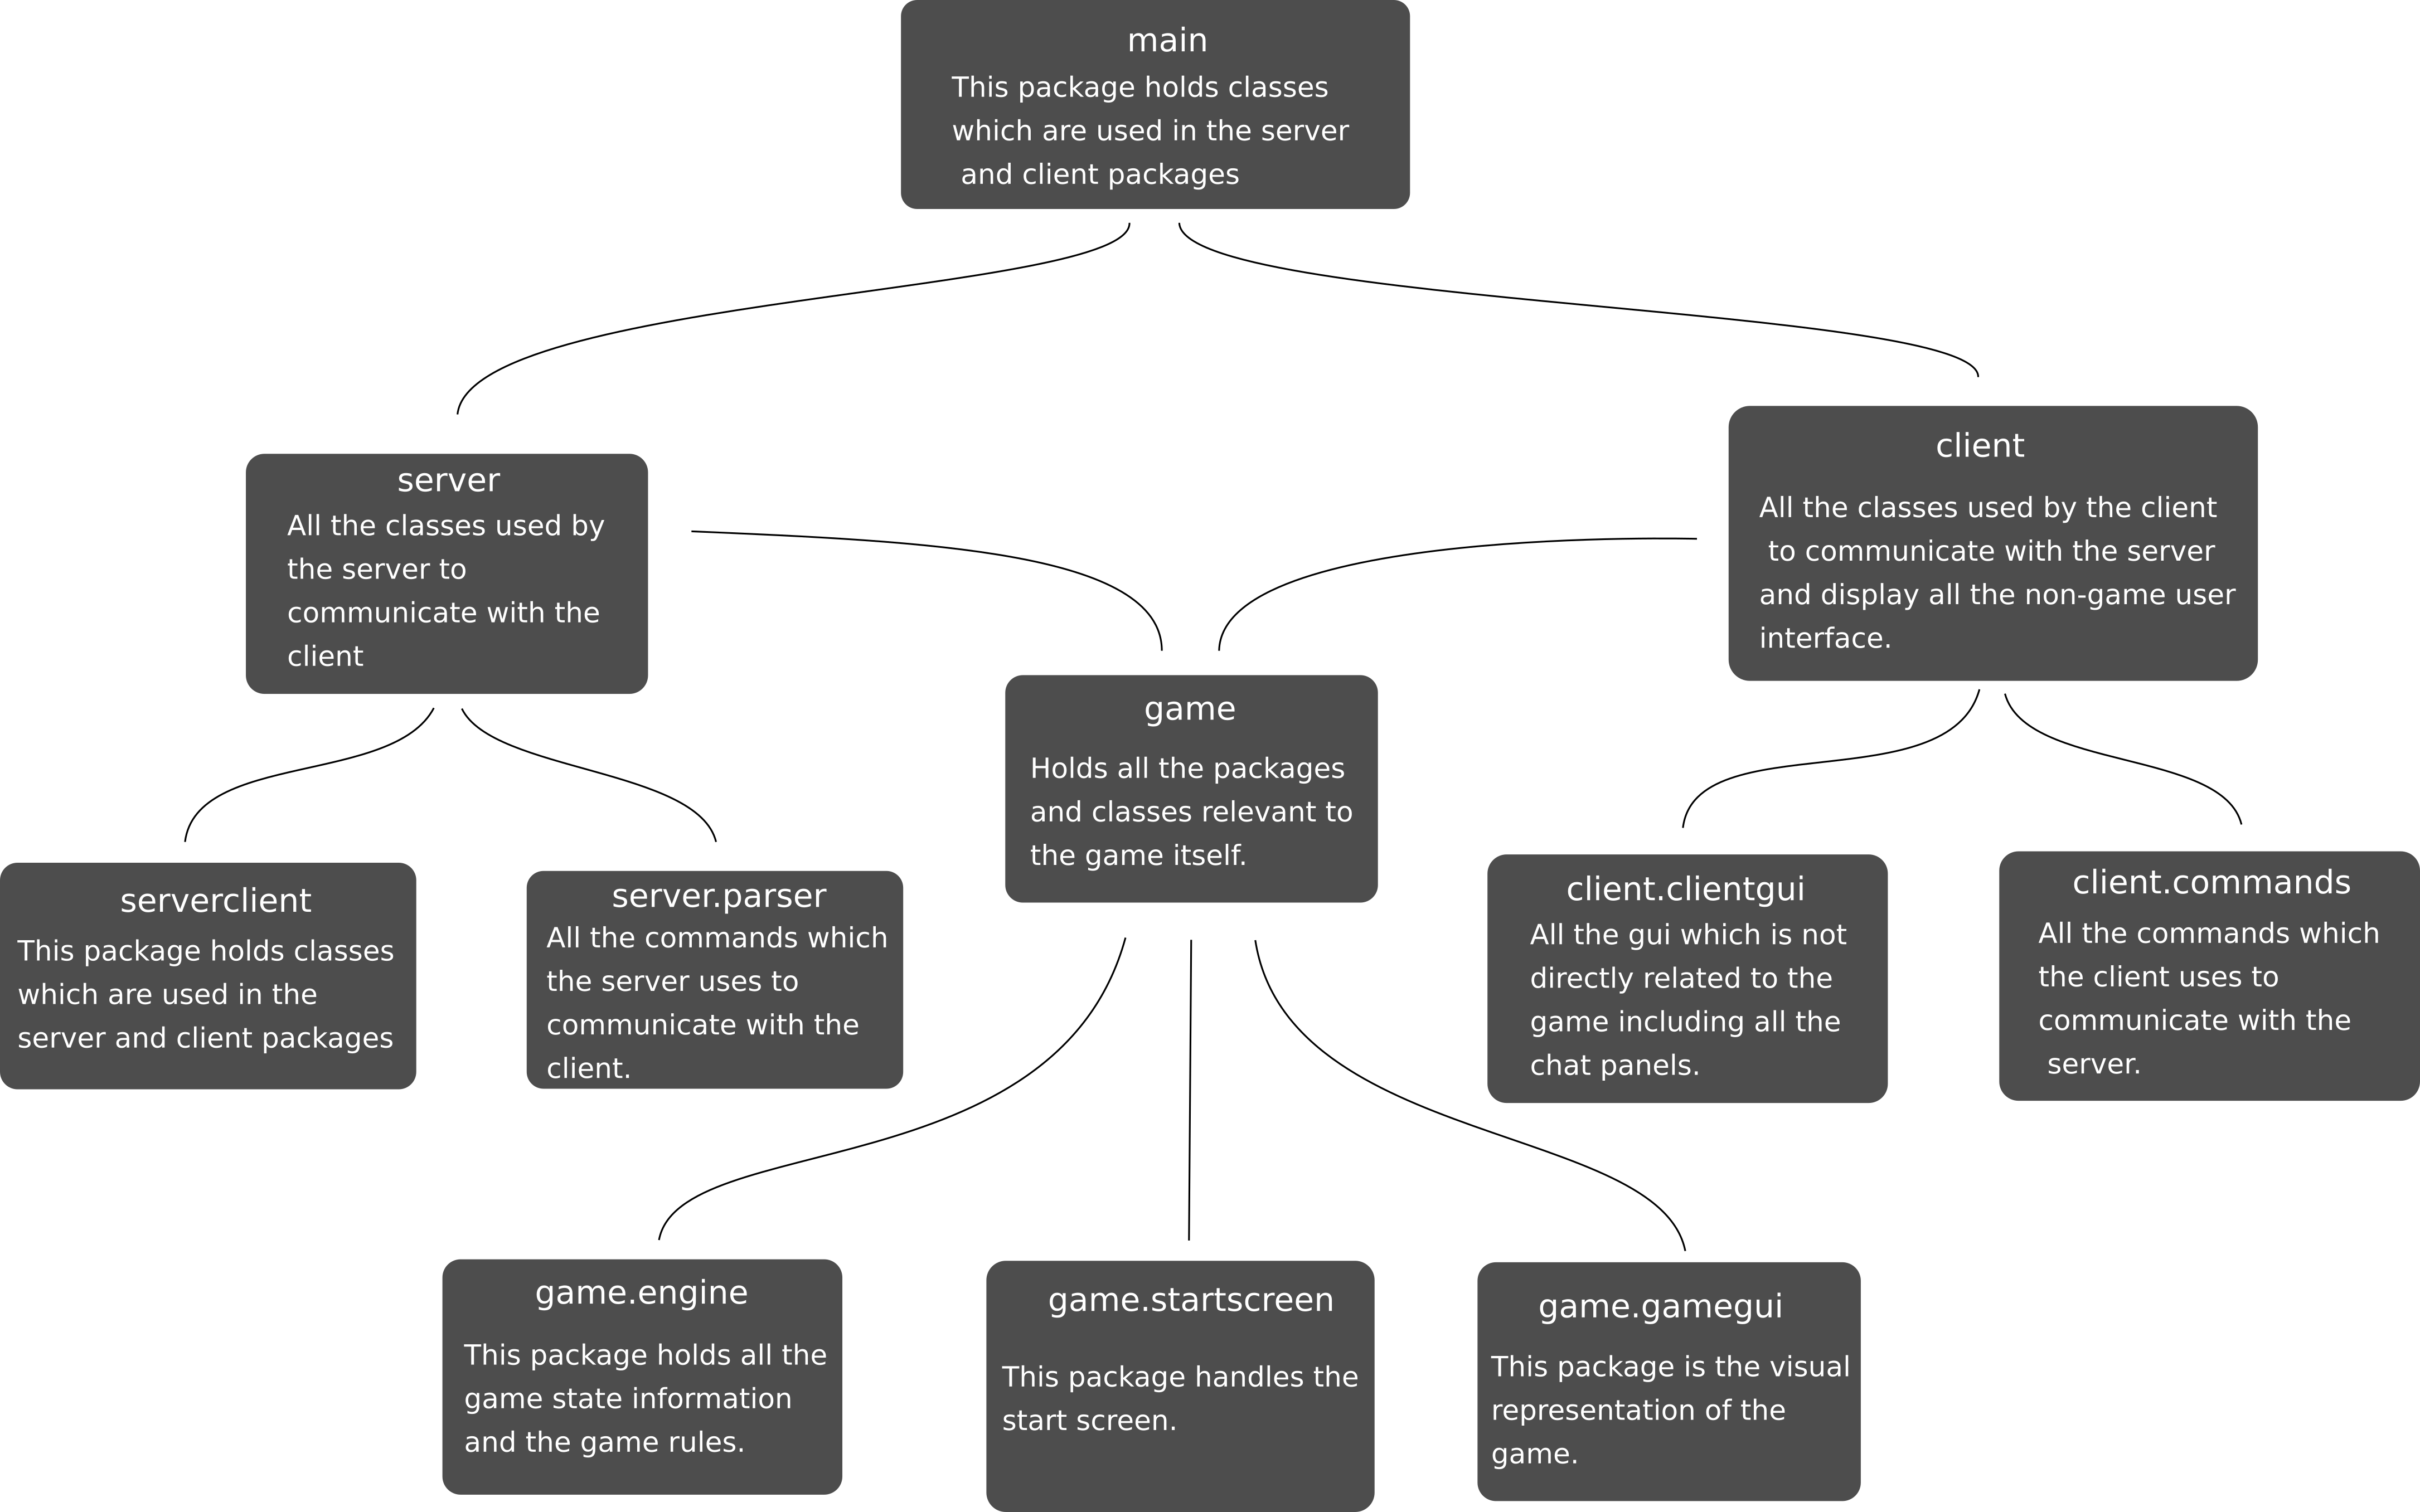
\includegraphics[width=140mm]{packages-hierarchie.png}
    		\caption{Overview of the package hierarchy used in the game}
    	\end{center}
    \end{figure}    
\end{document}
